
Put your Experimental results
\section{Testing Frame Construction(FrameObj)}
%Rebecca
% not sure how much of this le will go over...  :/
An easy way of being able to integrate with the other teams seemed to be through the creation of a class, FrameObj, which would not only provide the other modules with a means of creating a frame but a list of properties that could be called for easy debugging. In this object we can also store the values of constants and the ID numbers of devices, statuses, etc.  There are two ways that an instance of the class FrameObj could be constructed,  from the basic requirements of the frame (Frame type, Sender ID number , Receiver ID number, and Data) or from the bits of a frame.

FrameObj was written with a property, Listing \ref{propFrameObj}, for almost every field in the frame format. One notable exception is the data field of the frame. The property data is actually a combination of the data field and the CRC for the data. There are some additional properties as well; header and frameArray are not individual fields, instead they combine the fields of the entire header and frame respectively. The property classUse is not intended to be used outside the of the property data, it signifies which of the two ways of class initialization are used so that the data field can operate differently for either as well as for the different frameTypes.
\lstset{caption={Variable Properties of FrameObj},label=propFrameObj} 
\begin{lstlisting} 
    properties
        classUse    %Identifies which input configuration was used
        frameType   %Identifies the type of frame that is being used
        rcvID       %The identification number of the destination receiver
        sndID       %The identification number of the sender.
        data        %The data field (cuts off after more than 234 bytes)
        
    end
    properties (Dependent)
        dataSize    %Indicates the length of the payload in bytes.
        header      %The array of the frame header with hCRC8
        hCRC8       %CRC-8 code verfication of the header field
        dCRC8       %CRC-8 code verfication of the data field
        frameArray  %The frame as an n*1 array
    end
\end{lstlisting}

While writing FrameObj we also wrote the script FrameTest to test the various configurations under which FrameObj might be used. We tried to account for errors, both through using CRCs to protect our bits and by preparing for the rare errors that could happen and not result in an error with the CRC. FrameTest has been re-ordered in sections to best explain the current configuration of FrameObj and not to reflect the code development of FrameObj. The display statements in FrameTest showing the functionality of FrameObj can be found in Appendix \ref{FrameTestSrc} but are omitted here for clarity.

The first section of FrameTest shows the creation of an ACK frame. An ACK is a frame header with the frametype ACKFRAME. In FrameTest it is created from the frame constants: ACKFRAME, UEID1, and UEID2 with a zero entered instead of data.  
 
\lstset{caption={FrameTest Section 1: ACK},label=FrameTest1} 
\begin{lstlisting}
% create ACK
ACKtype = FrameObj(FrameObj.ACKFRAME, FrameObj.IDUE1, FrameObj.IDUE2, 0);
\end{lstlisting}

These constant properties correspond to the numbers 255, 101, and 102. Instead of just passing frameType=255 through the FrameObj (as we do with device ID numbers) we use a switch statement to compare the frameType input field to the six frameTypes used in FrameObj. The frameType is the most important property of our frame, it is the first part checked every time a frame is received. If a number is used that is not associated with a frameType it will result in a frame that is INVALID.

\lstset{caption={Function defining the frameType property of FrameObj},label=frameType} 
\begin{lstlisting} 
%frameType
        function obj = set.frameType(obj,inputframeType)
            %Using the switch statement in this way ensures that a
            %supported data type is used
            switch inputframeType
                case FrameObj.DATAFRAME     %DATA
                    obj.frameType = uint8(inputframeType);
                case FrameObj.ACKFRAME      %ACK
                    obj.frameType = uint8(inputframeType);
                case FrameObj.POLLFRAME     %POLL
                    obj.frameType = uint8(inputframeType);
                case FrameObj.REQFRAME      %REQ
                    obj.frameType = uint8(inputframeType);
                case FrameObj.TABLEFRAME    %TABLE
                    obj.frameType = uint8(inputframeType);
                case FrameObj.INVALID       %INVALID
                    obj.frameType = uint8(inputframeType);
                otherwise             % also INVALID
                    obj.frameType = uint8(FrameObj.INVALID);
            end
        end
\end{lstlisting}

Many of the other FrameObj properties depend on frameType. For instance ACK has no data CRC, as it has no data. For an FrameObj with frameType ACKFRAME, calling the property dCRC8 would result in an error, halting the program. Similarly, calling dCRC8 will result in an error, shown in Listing \ref{dCRC8}, if an unspecified frameType is used. This aids with frame creation. When an undefined frameType is used, errors will be triggered for each property that depends on frameType until that functionality is added. This way we can be sure that we are not using functionality assumed from other frameTypes. 

\lstset{caption={Function defining the dCRC8 property of FrameObj},label=dCRC8} 
\begin{lstlisting} 
%dCRC8
        %frameType dependent
        function value = get.dCRC8(obj)
            switch obj.frameType
                case FrameObj.DATAFRAME     %DATA
                    %The last byte of obj.data is the CRC. It is seperated
                    %from the data here
                    value = obj.data(end-8:end,1);
                case FrameObj.ACKFRAME      %ACK
                    error('This is an ACK, it has no data therefor no CRC')
                    %If there is no data there should be no check
					....
				otherwise
                    error('Not a supported frame type for dCRC8')
                    % If this error occurs while using a legitimate frame
                    % type please add an addiional case statement for that
                    % frame type.
\end{lstlisting}

No matter what type of valid frame is defined in FrameObj it will always have the same header format and length. The display messages in the command window shown in Figure \ref{fig:FrameTest1} confirm that there are 5 bytes of information in this ACK frame and the dataSize is hard-coded to 0. 

\begin{figure}[h]
    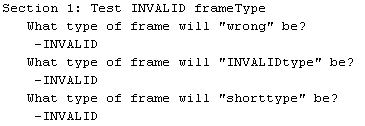
\includegraphics[width=0.5\textwidth, left]{FrameTest1.PNG}
    \caption{Command window output of FrameTest Section 1 showing ACK frame attributes }
    \label{fig:FrameTest1}
\end{figure}

The INVALID frameType is an important part of protecting the class FrameObj from error filled inputs especially when creating a FrameObj from transceived bits. Critical errors which would cause Matlab errors should result in an INVALID frame instead. In Section 2 of FrameTest, Listing \ref{FrameTest2}, we created three errors that resulted in INVALID frames, the output of this section is shown in Figure \ref{fig:FrameTest2}.

\lstset{caption={FrameTest Section 2: INVALID},label=FrameTest2} 
\begin{lstlisting} 
% nonsense frameType
INVALIDtype = FrameObj(20 , FrameObj.IDUE1, FrameObj.IDUE2, 0);

% cut off the number of bits
receivedshort = ACKtype.frameArray(1:39);
shorttype = FrameObj(receivedshort);

% adds 2000 zeros to the end of the bits 'correct'
% change the sender to IDUE3 to cause the CRC to have an error
receivedcbits = [ACKtype.frameArray; zeros(2000, 1)];
receivedcbits(2*8+1:3*8) =de2bi(uint8(FrameObj.IDUE3),8,'left-msb');
wrongcrc = FrameObj(receivedcbits);
\end{lstlisting} 

The first error, INVALIDtype in Listing \ref{FrameTest2}, is the most straight forward, instead of using a legitimate frametype as the first input to FrameObj, we used an invalid number: 20. This input will be passed to frameType where it will not match any of the defined switch cases in the property frameType from Listing \ref{frameType} and will be set to INVALID through 'otherwise'. The output is shown in Figure\ref{fig:FrameTest2}.  This is the only way to create an INVALID frame by using 4 input fields of FrameObj. 

\begin{figure}[h]
    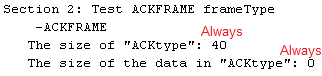
\includegraphics[width=0.9\textwidth, left]{FrameTest2.PNG}
    \caption{Command window output of FrameTest Section 2 showing that all three very wrong frames are INVALID }
    \label{fig:FrameTest2}
\end{figure}

The next two types of errors that result in INVALID frames are checked for in the FrameObj constructor, Listing \ref{FrameObj1} when the input is in bits. The first of these errors stems from the minimum size of a frame and therefore from the minimum acceptable length of the n*1 input. The array used in FrameObj, receivedshort from Listing \ref{FrameTest2},  must be at least 40 bits long to represent a valid frame. By defaulting all shorter inputs to INVALID we can be certain that we will not be indexing outside of the dimensions of the input. Figure \ref{fig:FrameTest2} shows that when the input has a length of only 39 bits the resulting frameType will be INVALID. 

\lstset{caption={Single bit array input constructor of FrameObj},label=FrameObj1} 
\begin{lstlisting} 
%Constructor, FrameObj with 1 array of bits
            elseif nargin == 1
                bitwise = inputType;
                 
                %size check
                [size_in, ~] = size(bitwise);
                if (size_in >= 40)
                    % hCRC check
                    hDetect = comm.CRCDetector([8 7 6 4 2 0]);
                    % detects if there is an error in the CRC of the header
                    [~, err] = step(hDetect, bitwise(1:5*8,1));
                    if (err ==0)
						....
                    else
                        % the crc does not match and the header is junk
                        obj.frameType = FrameObj.INVALID;
                    end
                else
                    % the data we recdived is not long enough to check the
                    % header crc
                    obj.frameType = FrameObj.INVALID ;     
                end
            else %incorrect number of inputs
                error('That is not a valid number of inputs')
            end
\end{lstlisting} 

The code from the FrameObj constructor in Listing \ref{FrameObj1}, shows the source of the last error that will result in an INVALID frame. After checking for the minimum size of the input, the constructor will check the CRC of the header. In FrameTest, Listing \ref{FrameTest2} we guarantee that the header will cause a CRC error by replacing the sndID number with another UEID number in the bit array receivedcbits. An error with the header CRC is not necessarily critical for the FrameObj construction but it is important for the functionality of the frame format in the network.

The data field of the frame format is the most complicated property to implement in FrameObj. Not only does it change dramatically with frameType but the way it functions changes with the way that FrameObj is used, with either 1 or 4 inputs. For an ACKFRAME frameType the data property must be initialized as a value or there will be an error but data should not be used. For a DATAFRAME frameType, data must either take in a string or an array of bits. Other frameTypes will have different requirements which means that very little processing can be done in the constructor of the FrameObj, the bulk of data must be defined in the property function. 

\lstset{caption={FrameTest Section 3: DATA },label=FrameTest3} 
\begin{lstlisting} 
str = [' abcdefghijklmnopqrstuvwxyz' char(10)]; %28 chars
str = [str str str];    % str is 28*3= 84 char long

%create the instance of FrameObj 'fromconst'
%adds 2000 zeros to the end of the bits 'fromconst'
fromconst = FrameObj(FrameObj.DATAFRAME,FrameObj.IDUE1,FrameObj.IDUE2,str);
receivedfrombits = [fromconst.frameArray; zeros(2000, 1)];

%create the instance of FrameObj 'frombits' which should be identical to
%'fromconst' 
%all trace of zero padding is gone
frombits = FrameObj(receivedfrombits);
\end{lstlisting} 

Section 3 of TestFrame, Listing \ref{TestFrame3}, tests the many aspects of the data creation of FrameObj as well as the dataSize. It does that by first properly creating the FrameObj fromconst and using the frameArray property to create the array of bits. With or without zero padding at the end, receivedfrombits can be used to create a FrameObj identical to fromconst in every way. Figure \ref{fig:FrameTest3} shows that every property of fromconst matches the corresponding property in frombits. The data property is only able to be found from the bitwise input when the dataSize is accurate.   

\lstset{caption={FrameTest Section 3: DATA },label=FrameTest3} 
\begin{lstlisting} 
%increase the size of str
str = [str str str]; % str is 84*3 = 252 bits long (over max size)
%create the instance of FrameObj 'long'
%adds 2000 zeros to the end of the bits 'long'
long= FrameObj(FrameObj.DATAFRAME, FrameObj.IDUE1, FrameObj.IDUE2, str);
\end{lstlisting} 
\begin{figure}[h]
    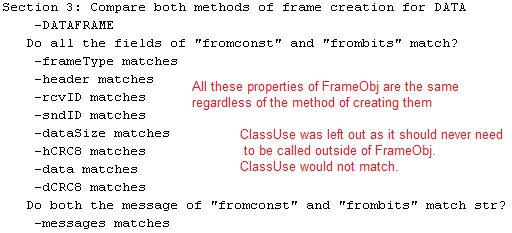
\includegraphics[width=0.77\textwidth, left]{FrameTest3.PNG}
    \caption{Command window output of FrameTest Section 3 showing an instances of FrameObj being created from both types of inputs }
    \label{fig:FrameTest3}
\end{figure}

The length the data field in all frameTypes is limited to a maximum of 234 bytes. Section 4 of FrameTest shows how errors in dataSize would be prevented from being greater than input dimensions. This will prevent Matlab errors but will not significantly increase the likelihood of the data being correct. In Listing \ref{FrameTest4.1} the size of the data input 'str' is increased from 84 bits long in Listing \ref{FrameTest3} to 252 bits. The data property should cut off 12 bits before adding on the CRC.

\lstset{caption={FrameTest Section 4: DataSize },label=FrameTest4} 
\begin{lstlisting} 
%increase the size of str
str = [str str str]; % str is 84*3 = 252 chars (over max size)
%create the instance of FrameObj 'long'
long= FrameObj(FrameObj.DATAFRAME, FrameObj.IDUE1, FrameObj.IDUE2, str);

% create frankenstein's frame (so the we won't make an INVALID frame)
receivedbits1 = [long.header; fromconst.data];
DScheck1 = FrameObj(receivedbits1);

% create frankenstein's frame (with 1 extra zero)
receivedbits2 = [long.header; fromconst.data; 0 ];
DScheck2 = FrameObj(receivedbits2);

% create frankenstein's frame
receivedbits3 = [fromconst.header; long.data];
DScheck3 = FrameObj(receivedbits3);
\end{lstlisting} 

To compare the length of the message within data with the length of str as seen in Figure \ref{fig:FrameTest4}, we used DataMessage, Appendix \ref{DataMessage} to convert the bits back into characters.  Figure \ref{fig:FrameTest4} shows that str and the data message are no longer the same length as a result of the limit on the size of the data field. In the following subsections of section 4 the dataSize will be tested at both higher and lower values then corresponds to the data property passed to the FrameObj. We do this by creating frakenstein's frames from the header of one frame and the data of another. 

\begin{figure}[!]
    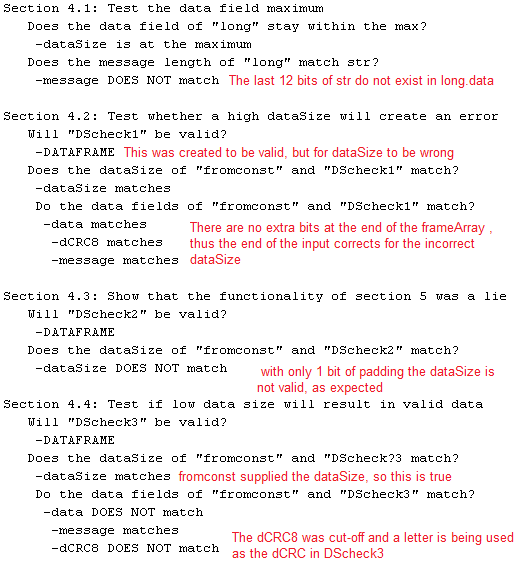
\includegraphics[width=0.8\textwidth, left]{FrameTest4.PNG}
    \caption{Command window output of FrameTest Section 4 showing dataSize limits  }
    \label{fig:FrameTest4}
\end{figure}

The subsections 2 and 3 of Listing \ref{FrameTest4} uses the same header and data properties to create the new FrameObjs DScheck1 and DScheck2. Both use data sizes longer than the message in the data property. The difference is that DScheck2 contains one additional zero at the beginning. This single bit of zero padding is the difference between data with a dCRC8 in DScheck1 which will check out without error and the dCRC8 in DScheck2 which does not match the original.  

\section{End-to-End Local Machine Testing }
%Renato
The test of the implementation of the end to end communication.
Based on proposal of final design project \cite{cdproj}, there
are six case to be tested in the end to end communication
\begin{enumerate}
  \item Extra-cellular communications between UEs
  \begin{enumerate}
    \item US1 $\rightarrow$ BS1 $\rightarrow$ BS2 $\rightarrow$ US3
    \item US3 $\rightarrow$ BS2 $\rightarrow$ BS1 $\rightarrow$ US1
		\item US2 $\rightarrow$ BS1 $\rightarrow$ BS2 $\rightarrow$ US3
		\item US3 $\rightarrow$ BS2 $\rightarrow$ BS1 $\rightarrow$ US2
  \end{enumerate}
  \item Intra-cellular communications between UEs
	  \begin{enumerate}
    \item US1 $\rightarrow$ BS1 $\rightarrow$ US2
    \item US2 $\rightarrow$ BS1 $\rightarrow$ US1
	\end{enumerate}
\end{enumerate}

The figure \ref{fig:endendDiagram} shows how the whole MATLAB code is organized to test the cases described in this section.
The send and received parts map each path of information from a UE  to a BS as a channel.  It is a logical representation of the physical channels for the end-to-end implementation in the final integration.
The routing used was just a switch case based on picture of proposed network in \cite{cdproj}.
The send and received is a recursive function that calls itself based with parameters changed for the routing.
One examples is shown in Listing \ref{sendReceiveExample} shows how once inside a channel it will resend the message or exit the the function based on the destination.
\lstset{caption={Code examples how to verify the CRC and create the ACK message back to sender},label=sendReceiveExample}
\lstinputlisting{code/sendReceiveExample.M}

The Listing \ref{crcVerification} is a examples how the receiver UE in the Figure \ref{fig:endendDiagram} verifies the data CRC and creates the new ACK frame to send back.
This procedure is important because it needs to be done in the integration with other teams that need to use the frameObj.     

\lstset{caption={Code examples how to verify the CRC and create the ACK message back to sender},label=crcVerification}
\lstinputlisting{code/crcVerification.M}



\begin{figure}[ht]
    \centering
    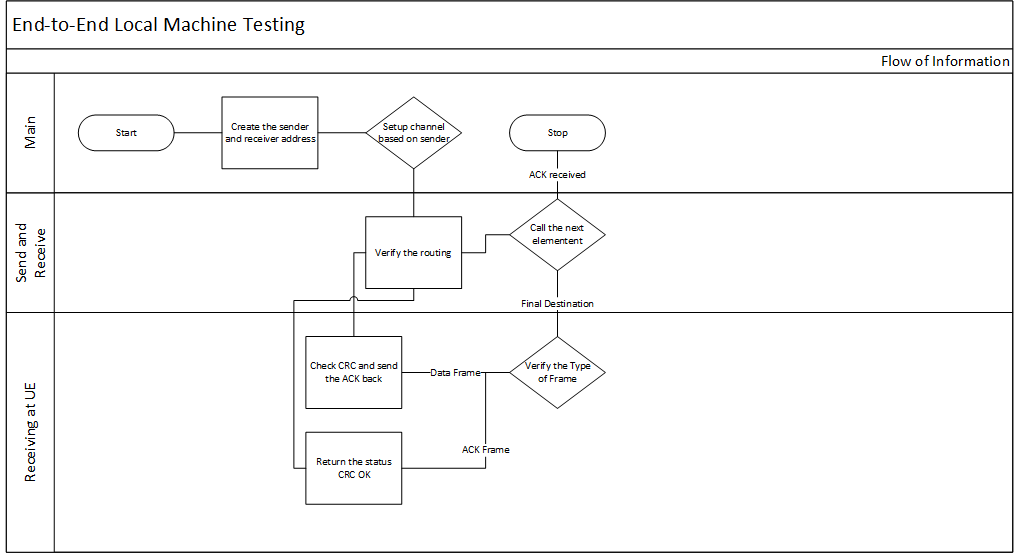
\includegraphics[width=0.8\textwidth]{flowEndtoEnd.PNG}
    \caption{Diagram of the flow of information to test the end to end in Matlab for the team 6 proposed protocol}
    \label{fig:endendDiagram}
\end{figure} 

\section{Transmitting and receiving over the air}
%Renato
The frame object needs to be tested over the air to check if it behaves as expected in our simulation. 
It was tested using two different physical layers. 
\subsection{Using lab2 physical layer}

The first test was using a very straight forward approach. We just replaced the 'hello world' message in the Lab 2 
simulating model to add the FrameObj with a message 'Hi', so it can send a frame near the original size (88 bit versus 64 bits).
The code to create a frame is shown in \ref{transLab02}. It is used as input of simulation in diagram of Figure \ref{fig:trasmitter_lab02}.

\lstset{caption={Code to create the transmitter package to used in Lab 02 physical layer},label=transLab02}
\lstinputlisting{code/crcVerification.M}

\begin{figure}[ht]
    \centering
    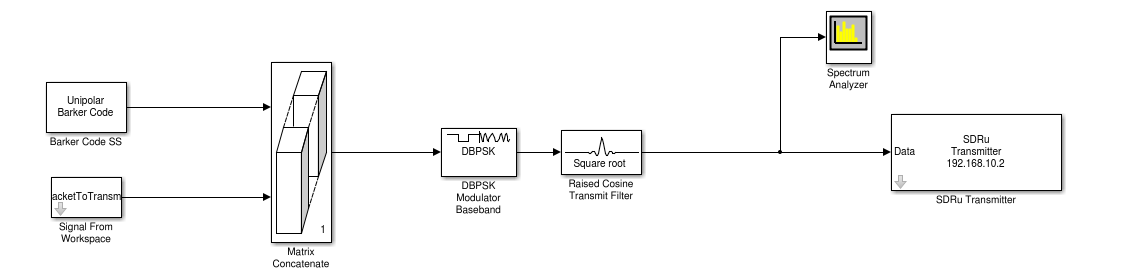
\includegraphics[width=0.8\textwidth]{trasmitter_lab02.PNG}
    \caption{Simulink diagram of the laboratory two physical layer transmitter modified to received a FrameObj with the message 'Hi' }
    \label{fig:trasmitter_lab02}
\end{figure}

The receiver changed also to verify the data CRC and count the number of DATAFRAMEs,ACKFRAMES and INVALID frame that were received. The diagram of this receiver is
shown in Figure \ref{fig:receiver_lab02}.

\begin{figure}[ht]
    \centering
    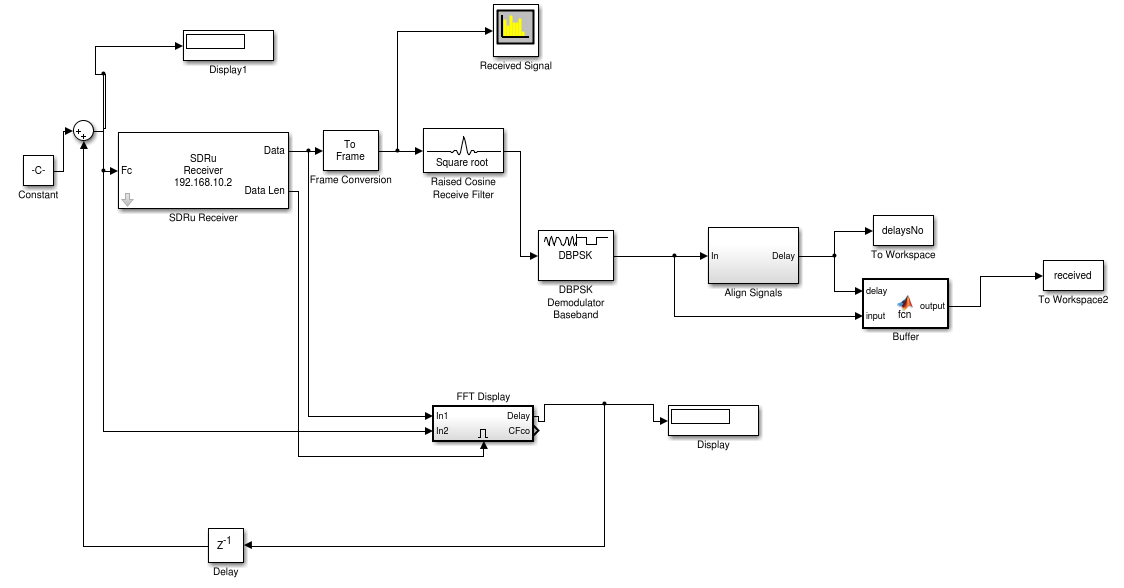
\includegraphics[width=0.8\textwidth]{receiver_lab02.PNG}
    \caption{Simulink diagram of the laboratory two physical layer receiver modified to received a frame and verify the CRC and frameType }
    \label{fig:receiver_lab02}
\end{figure}


The result was very poor. The table \ref{tab:2ACK} shows a FER around 97\% and there were 2 cases of the false detection of an ACK frame when the transmitter only sent
the same data frame with the message 'Hi'.  


To avoid the false detection, we change the value of the DATAFRAME to 240 (1111 0000 in binary) and the ACKFRAME to 255 (1111 1111 in binary).
The FER was still very high, above 95\%, but no ACKFRAMEs were detected as shown in Table \ref{tab:0ACK}. Increasing the hamming distance betweenthe numerical representation of DATAFRAME and ACKFRAME
fixed this false detection.
 
\begin{table}[ht]
	\centering
		\begin{tabular}{| c | c | }
		\hline                       
		Frame Type UE & Number Received\\
		\hline
			ACK & 2\\
			DATA & 102\\
			corrupt DATA & 2\\
			INVALID & 3466\\
			other & 0\\
		\hline
		\end{tabular}
	\caption{Table of frames received with poor transmission quality and a small hamming distance between frame types.The ACK was a false positive error because the frameTypes were very similarr numbers}
	\label{tab:2ACK}
\end{table}

\begin{table}[ht]
	\centering
		\begin{tabular}{| c | c | }
		\hline                       
		Frame Type & Number Received\\
		\hline
			ACK & 0\\
			DATA & 165\\
			corrupt DATA & 4\\
			INVALID & 3559\\
			other & 0\\
		\hline
		\end{tabular}
	\caption{Table of frames received with poor transmission quality and a larger hamming distance between frameTypes}
	\label{tab:0ACK}
\end{table}
\subsection{Using Team 4 physical layer}
\label{team4_results}
To decrease the FER, we replaced the Lab two physical layer for one more robust. Interleaving and bit repetition would improve the recovery of the information in the receiver side.
We used the transceiver from Team 4  which included those types of coding but needed minor modification to transmit the FrameObj instead of the frame from Team 4.
The first modification was to re-size the block interleave to handle an 8 bit word instead of the 7 bit words used by Team 4. We also changed the size of the zero-padding, our message was smaller and we decide to keep the same output of 987 bits to add to the13 bit Barker code. The diagram of this transmitter is shown in Figure \ref{fig:transmitter_team4}. It is very similar to the one from laboratory 02,  the main change is the size of buffer to fit the repeated and interleaved message. 
 
\begin{figure}[ht]
    \centering
    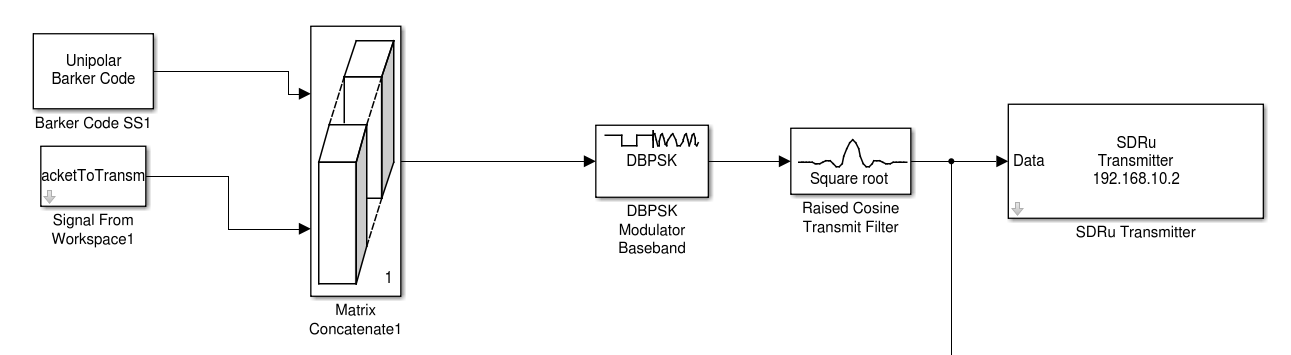
\includegraphics[width=0.8\textwidth]{transmitter_team4.PNG}
    \caption{Simulink diagram of the receiver of the laboratory two physical layer modified to received a a frame and verify the CRC and which frame type }
    \label{fig:transmitter_team4}
\end{figure}

The receiver diagram from figure \ref{fig:receiver_team4} is much more complex from laboratory 02 because Team 4 upgrade the delay detection and the frequency correction.
We made similar changes to the receiving interleaver as to the transmiting interleaver and get the mean of the values of the repeated bits to recreate the DATAFRAME FrameObj.
We also make the bi-directional transmission. We receive the DATAFRAME check of the dCRC8. The performance of receiving data package is show in Table \ref{tab:team4data}. If at least one data packet is correct, we start the transmitter block in figure \ref{fig:transmitter_team4} to send the ACKFRAME back to the other machine. The performance of receiving ACK package is shown in Table \ref{tab:team4ack} . The fulll code for this receiver is shown by the listing \ref{ReceiverTeam4Code} in the appendix. This process was recoded and is available at \cite{videodemo}. 
 

\begin{figure}[ht]
    \centering
    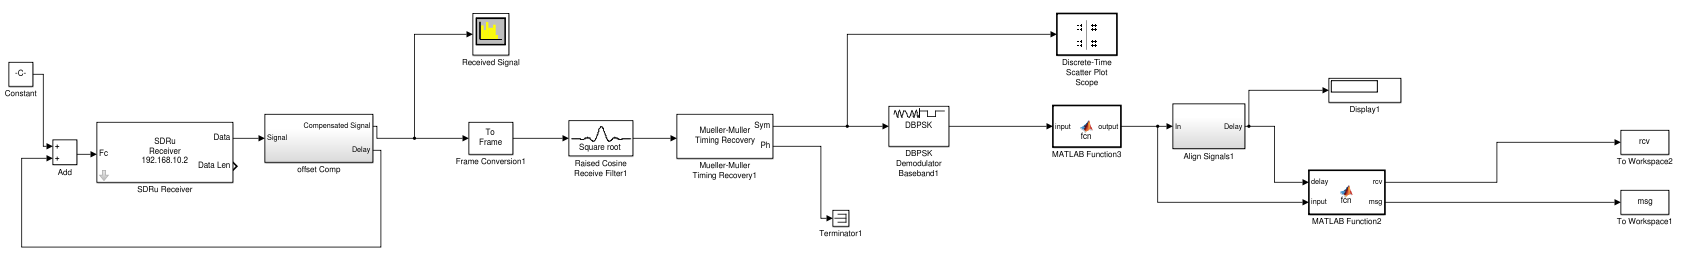
\includegraphics[width=0.8\textwidth]{receiver_team4.PNG}
    \caption{Simulink diagram of the Team 4 receiver modified to received a FrameObj and verify the CRC and frameType }
    \label{fig:receiver_team4}
\end{figure}

\begin{table}[ht]
	\centering
		\begin{tabular}{| c | c | }
		\hline
			\multicolumn{2}{|c|}{Data Frame}\\
		\hline                       
			 Total frame received & 62\\
			 Correct frame received& 23\\
		\hline
			FER & 63\%\\
		\hline
		\end{tabular}
	\caption{Table of data frames received using the team 4 physical layer with repetition factor of 4 and block interleaving}
	\label{tab:team4data}
	\end{table}

\begin{table}[ht]
	\centering
		\begin{tabular}{| c | c | }
		\hline
			\multicolumn{2}{|c|}{ACK Frame}\\ 
		\hline                       
			 Total frame received & 66\\
			 Correct frame received& 37\\
		\hline
			FER & 44\%\\
		\hline
		\end{tabular}
	\caption{Table of ack frames received using the team 4 physical layer with repetition factor of 4 and block interleaving}
	\label{tab:team4ack}
	\end{table}
